\documentclass[11pt,a4paper]{jsarticle}

\usepackage[dvipdfmx]{graphicx}
\usepackage{graphicx}
\usepackage[top=20truemm,bottom=20truemm,left=25truemm,right=25truemm]{geometry}
\usepackage{comment}

\usepackage[hang,small,bf]{caption}
\usepackage[subrefformat=parens]{subcaption}
\captionsetup{compatibility=false}

%https://qiita.com/Toru3/items/7ea1342da1e31f0c28c3
\usepackage{fancyhdr}
\usepackage{lastpage}
\fancypagestyle{mypagestyle}{%
\lhead{\thepage/\pageref{LastPage}}%ヘッダ左
\rhead{研究論文の要旨2 (卒業研究中間報告書の要旨) 平松信義}%ヘッダ右
\cfoot{}%\thepage/\pageref{LastPage}}%フッタ中央に"今のページ数/総ページ数"を設定
\renewcommand{\headrulewidth}{0.0pt}%ヘッダの線を消す
}
\pagestyle{mypagestyle}

\title{研究論文の要旨2 (卒業研究中間報告書の要旨)\\研究テーマ: IrTe$_2$における準安定な超伝導相の光誘起}

\author{東京大学工学部物理工学科 賀川研究室 平松信義}
\date{\today}
\begin{document}
\maketitle
\thispagestyle{mypagestyle}


\section{はじめに}
%相転移/急冷/超伝導/鉄鋼/強相関電子系/準定常状態の電流励起/電荷秩序と競合した超伝導相
超伝導とはある温度以下で電気抵抗がゼロになる現象で、1911年にオランダのオンネスが発見した。多彩かつ応用上有利な性質を超伝導物質は示すため、現在まで様々な超伝導物質に関して活発な研究開発が進められてきた。特に1986年に銅酸化物高温超伝導体が発見されて以来、特に銅酸化物を含む強相関電子系と呼ばれる物質群は精力的な研究の対象となった。

強相関電子系を特徴づける電子間の相対的に強い反発力は、超伝導を発現することがある一方で、電荷やスピンなどの秩序化も担う。これらの超伝導相と秩序相は起源を同じくするため、物質中で競合または共存\cite{Fausti,2D_SC}しており、一方の理解は他方の理解にも繋がる。また超伝導の前駆状態として秩序相が現れている可能性も示唆されている\cite{Valla1914}。したがって新しい超伝導物質や超伝導状態の開拓のためには秩序相の理解が有益である。

遷移金属カルゴゲナイドIrTe$_2$は低温で構造相転移し電荷が一次元的に配列する電荷秩序状態(電荷密度波)となるが、
この物質にパラジウム(Pd)を添加すると臨界温度3Kで超伝導を示す\cite{IrTe2Pd_SC}。この系は大きなスピン-軌道相互作用に起因して、非従来型の超伝導物質として注目されている。近年、電荷秩序状態にある薄膜のIrTe$_2$試料に電流パルスを印加すると、試料の急冷が起こり秩序相が破壊され、競合する超伝導状態が現れることが実験により示された\cite{SC_IrTe2}。この研究は急冷により電子の相を制御し超伝導を発現できることを示した点で画期的だと筆者は考える。しかし電流パルス印加では試料の冷却速度に上限がある。またこのような急冷後に現れる超伝導相に関しては、いまだ理解されていないことが多い。

本研究の目的はIrTe$_2$の超伝導状態をレーザーパルス光を用いた急冷から誘起できることを示し、その超伝導状態が実現される過程の理解を深めることである。パルス光を用いると試料の高速な加熱・冷却が可能であり、より多くの物質に関して超伝導を発現できる期待がある。また光を用いるとパターニングされた超伝導回路を、試料上に繰り返し書き込みすることが可能になり、幅広く応用の可能性を考えられる。

筆者は超伝導状態を光誘起するために、パルス光を試料に入射できる偏光顕微光学系を構築した。そしてその光学系で試料を観察しながら超伝導状態を光誘起することを目標とした。筆者はまずパルス光を入射する前の予備実験として、光学クライオスタット内のIrTe$_2$試料の抵抗を測定しながら温度を変化させ、偏光顕微鏡によって試料の秩序相を観察した。本報告書ではその予備実験によって得られた成果と今後の課題について報告する。

\section{実験方法}
IrTe$_2$試料は理化学研究所の上谷研究員から提供を受けた。試料は電気端子を接続してから光学クライオスタット内に格納し、試料の温度をヘリウム冷凍機とヒーターを用いて制御した。そして試料の抵抗を測定しながら温度を変化させ、偏光顕微鏡によって試料を観察した。

\section{実験結果}
試料の相転移を観察するために、試料の温度を300Kから50Kまでレート1K/minで冷却したあと、同一のレートで50Kから300Kまで加熱した。図\ref{fig:resistance50-300}に抵抗の温度に関するヒステリシス曲線を示す。冷却中は270K付近と110K付近で、不連続に抵抗が増加した。加熱中は280K付近で不連続に抵抗が減少した。また240K付近で特徴的な抵抗の増加が見られる。抵抗の不連続な変化に対応して、偏光顕微鏡写真は定性的に大きく変化した。

図\ref{fig:nonpolv250}と図\ref{fig:nonpolv100}に、温度250Kと100Kで撮影した偏光顕微鏡写真をそれぞれ示す。図\ref{fig:nonpolv250}と図\ref{fig:nonpolv100}は試料の対応する領域を、同一の実験条件で撮影したものである。光学系から偏光子を取り外した条件で撮影した。

図\ref{fig:nonpolv250}から反射光の強度が大きい(明るい)領域と反射光の強度が小さい(暗い)領域が明瞭に見て取れる。明るい領域は異方的な構造を持つことが分かる。明るい領域と暗い領域の境界は三方向に伸びており、それらの方向はお互いに概ね角60度をなしていた。さらに繰り返し実験を行うと相転移後の明暗のパターンは毎回異なり、再現しないことが分かった。以上で述べたような明暗のパターンは300Kの顕微鏡写真では見られなかった。

図\ref{fig:nonpolv100}(100K)を図\ref{fig:nonpolv250}(250K)と比較すると、明暗のパターンが変化したことがわかる。また100Kではコントラストが小さくなった。100Kの顕微鏡写真に特徴的な明暗のパターンは、加熱しても元に戻らず290Kまで保たれた。

\begin{figure}[h]
  \begin{center}
   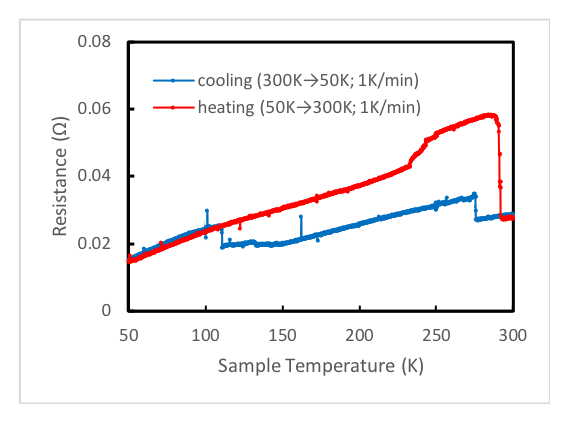
\includegraphics[width=0.7\hsize]{resistance50-300.eps}
  \end{center}
  \caption{抵抗の温度依存性}
  \label{fig:resistance50-300}
\end{figure}
 \begin{figure}[h]
 \begin{minipage}{0.5\hsize}
  \begin{center}
   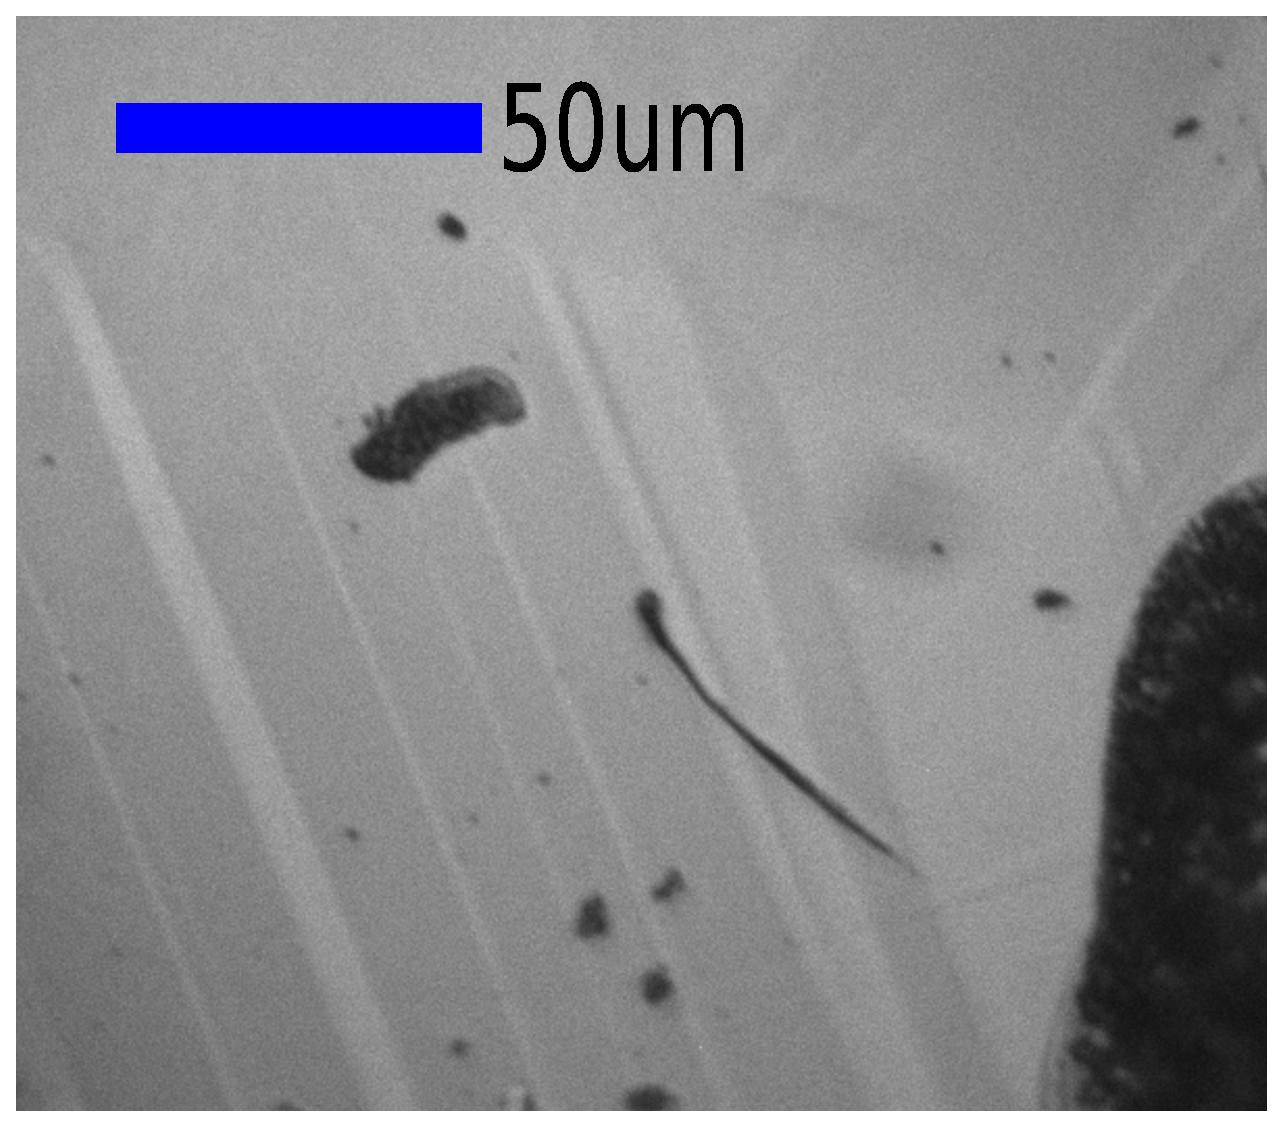
\includegraphics[width=0.95\hsize]{nonpolv250.eps}
  \end{center}
  \subcaption{250K}
  \label{fig:nonpolv250}
 \end{minipage}
 \begin{minipage}{0.5\hsize}
  \begin{center}
   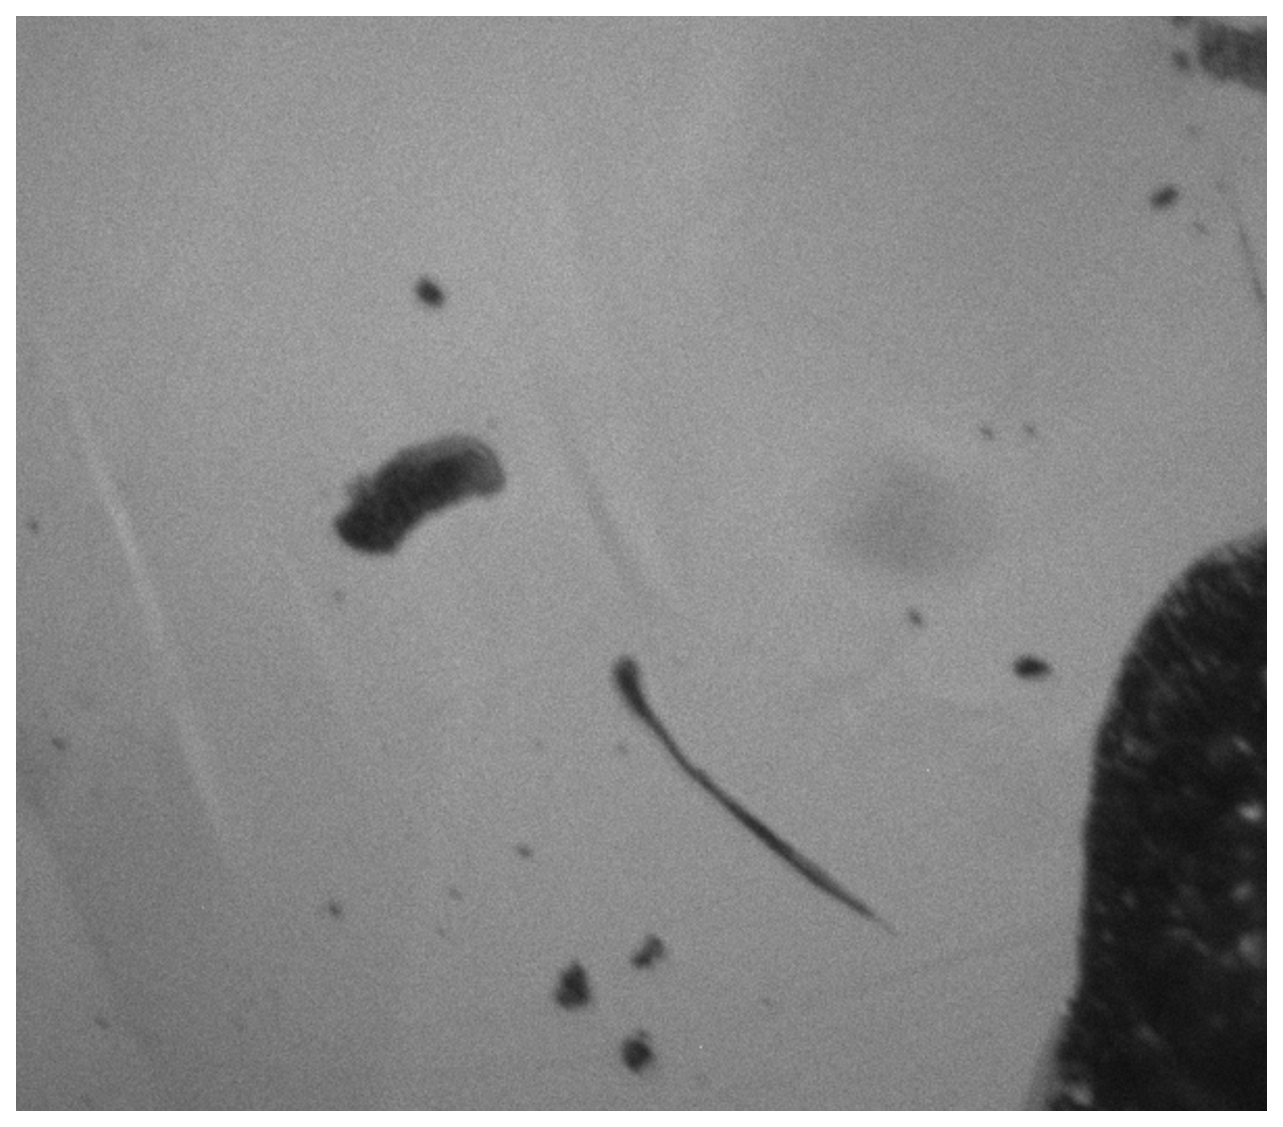
\includegraphics[width=0.95\hsize]{nonpolv100.eps}
  \end{center}
  \subcaption{100K}
  \label{fig:nonpolv100}
 \end{minipage}
  \caption{バルクIrTe$_2$試料の偏光顕微鏡像}
\end{figure}



\section{議論}
試料を300Kから冷却してゆくと280K付近で抵抗が不連続に変化し、顕微鏡像に明暗のパターンが現れた。この明暗のパターンは300Kの高温相では見られなかった。これらの結果は少なくとも一部の領域に低温相が現れた証拠である。また実験からこの相が異方的であることを確かめた。明るい領域と暗い領域の境界が三方向に伸びている結果は、高温相の結晶の三回回転対称性を反映したものである。さらに本実験から、低温相への転移後の明暗のパターンが繰り返し再現しないことが分かった。相転移時に低温相の核ができる位置が繰り返しごとに異なることを意味し、核生成が確率的な事象であることを示唆すると筆者は考える。

試料を250Kから冷却してゆくと110K付近で、さらに抵抗が不連続に変化し、顕微鏡像の明暗のパターンが変化した。低温相が異なる第二の低温相にさらに相転移した証拠だと筆者は考える。冷却中に110K付近で現れた相の顕微鏡写真に特徴的な明暗のパターンは、加熱してゆくと遅くとも250Kでも保たれた。このような特徴的なヒステリシスの効果は先行研究\cite{IrTe_TT3,IrTe_TT4}でも確認されている。110Kで現れた相が先行研究で示されたような第二の低温相であるとの考えを、裏付ける。
 
 \section{結論}
筆者はバルクIrTe$_2$試料を温度変化させながら偏光顕微鏡で観察した。
300Kから除冷してゆくと偏光顕微鏡写真から、280K付近で異方性のある相が現われ、さらに110K付近で異なった相が現れることを確認した。偏光顕微鏡写真から、バルクIrTe$_2$試料の秩序相とその相転移を観察できたこの成果は、今後超伝導相をよりよく理解するために有益である。これまでの実験で得られた知見から光学系を改良し、超伝導状態の結晶の相をより明らかに同定できるように実験を進めていきたい。

\bibliography{zenki_jikken.bib}
\bibliographystyle{junsrt}


\end{document}
%コンパイルの仕方
%1. texファイルを一回コンパイル
%2. bibファイルを一回コンパイル
%3. texファイルを三回コンパイル